\chapter{Introduction} \label{intro}

Twenty-five years ago, the Nobel Prize-winning discovery of an exoplanet, a planet outside of our solar system, orbiting a Sun-like star shook the astronomical community and amplified a wave of exoplanet science that thrives to this day. \citet{mayor_jupiter-mass_1995} detected the planet indirectly by measuring the motion of the planet's host star over time, rather than the planet itself, using what is called the radial-velocity technique. These measurements required a high-resolution spectrograph---an instrument that can measure the electromagnetic spectrum of the star to high precision---taking stellar light, coupled via optical fiber, from a telescope at the Haute-Provence Observatory in France \citep{baranne_elodie_1996}.

With this technique and instrument, they were able to detect 51 Pegasi b, a planet about 150 times more massive than Earth with an orbit closer than that of Mercury. It is quite a testament that, more than two decades later, we are at the breaking point of using the radial-velocity technique with ground-based fiber-fed spectrographs---essentially the exact same methodology and technology---to discover Earth-mass planets orbiting within their host star's habitable zone.

In this thesis, I describe my personal contributions towards the technological advancements necessary to detect exoplanets at such extreme precision. These advancements encompass multiple approaches to technology development, from instrument design and the mitigation of physical noise sources to the implementation of novel data analysis algorithms. Such a holistic approach towards instrumentation has been crucial in clarifying the steps required to reach the next generation of exoplanet measurement. Through this introduction, I aim to demystify some of the terminology surrounding my research and reveal some of the links between various aspects of my work.

\section{The Radial-velocity Technique} \label{intro:eprv}

The principles of the radial-velocity technique are built upon two fundamental concepts in physics: Newton's Third Law of Motion and the Doppler Effect. As a planet orbits around its host star, held in by the star's gravitational pull, the planet itself imparts an equal but opposite gravitational force on the star. Thus, both the planet and the star follow similar orbits around the center of mass of this two-body system. If we can measure orbit-like periodicity in the motion of the star, we can therefore infer the existence of an exoplanet \citep{lovis_radial_2011}. Importantly, the motion we choose to measure is the stellar \textit{radial} velocity (RV)---movement directly towards and away from us, the observer---rather than any \textit{transverse} velocity (up, down, left, or right), which we leave to the field of astrometry.

But how does one actually measure a stellar RV? Using the Doppler Effect! As light is emitted from the star (and before it takes a multi-year journey to Earth), the relative motion of the star causes the physical characteristics of this light to change depending on how the star is moving. If the star is moving towards Earth (with negative velocity $v$), the frequency ($f$) of the light increases (equivalent to saying the wavelength $\lambda$ of the light decreases) and is therefore called blue-shifted since higher frequency light appears bluer to the human eye. If the star is moving away from Earth (positive $v$), the light is oppositely called red-shifted ($f$ decreases, $\lambda$ increases). These shifts in frequency can be subsequently converted into relative RV measurements of the star using the relativistic Doppler equation
\begin{equation}
    \frac{f_o}{f_s} = \frac{\lambda_s}{\lambda_o} = \sqrt{\frac{1 - v/c}{1 + v/c}}
    \label{eq:relative-doppler-effect}
\end{equation}
where $o$ and $s$ represent measurement at the observer (Earth) and source (star) respectively, while $c$ is the speed of light in a vacuum. Therefore, the more precise goal of using the RV technique is to measure light from the star at many points in time, calculate the blue/red-shift of the light at each time, and convert these shifts into RVs.

This leaves us now with two questions: (1) How do we ``measure light'' from a star? (2) What can we actually do with these stellar RVs? I'll start by answering the second of these questions first.

\subsection{The Keplerian RV Model}

Time series of stellar RVs can be used to infer parameters that describe a planet and its orbit around its host star. These parameters include, most critically, the mass of the planet and its orbital period, the time it takes to complete one full rotation around the star. However, it takes a bit of physics and math to derive where this information comes from.

I'll start by describing the elements of a Keplerian orbit, typically written as
\begin{equation}
    r(\theta) = \frac{a (1-e^2)}{1 + e \cos{\theta}}.
    \label{eq:kepler}
\end{equation}
At any given angle $\theta$ within an orbit---also known as the true anomaly from periapsis, the position of closest approach to the center of mass of the system---the distance $r$ from the center of mass can be described as an ellipse with semi-major axis $a$ and eccentricity (or elliptical elongation) $e$. An orbit with $e=0$ is completely circular, since it would mean $r(\theta)=a$.

However, RV measurement is limited to velocity, rather than positional, data and we are stuck viewing the orbit from an arbitrary (and typically unknown) angle. Therefore, we rewrite the Keplerian model as
\begin{equation}
    v(t) = K (\cos{(\theta(t)+\omega)} + e \cos{\omega})
    \label{eq:kepler-rv}
\end{equation}
where $\omega$ is the argument of periapsis---a constant angle that describes the orientation with which we are viewing the orbit based on the position at periapsis---and $K$ is what we call the RV semi-amplitude \citep{lovis_radial_2011}.

You may notice that the true anomaly $\theta(t)$ is now represented as a function in time ($t$). Since RV data is taken through a series of observations at different moments in time, time is the natural independent variable in our model. Through a couple of steps, we can map out the relationship between $\theta$ and $t$:
\begin{equation}
    \theta(t) = 2 \arctan{\left(\sqrt{\frac{1+e}{1-e}}\tan{\left(\frac{E(t)}{2}\right)}\right)}
    \label{eq:mean-anomaly}
\end{equation}
where the eccentric anomaly $E(t)$ (an intermediate way of describing the orbital angle) has a transcendental (not analytically solvable) relationship to the times of observation:
\begin{equation}
    E(t) - e \sin{E(t)} = \frac{2\pi (t - \tau)}{P}.
    \label{eq:eccentric-anomaly}
\end{equation}
$\tau$ is the time of pariapsis, or the time at which the orbit sits at the angle $\omega$, and $P$ is the period of the orbit.

Along with the time-dependent angle $\theta(t)$, the other important aspect of Equation \ref{eq:kepler-rv} is the constant RV semi-amplitude $K$. This value is the maximum RV of the star as it moves towards and away from the observer and can be rewritten in terms of other orbital parameters:
\begin{equation}
    K = \frac{2\pi a_* \sin{i}}{P\sqrt{1-e^2}}
    \label{eq:rv-semi-amplitude}
\end{equation}
where $a_*$ is the semi-major of axis of the stellar orbit and $i$ relates to the inclination of the orbit from the observer's perspective. Note that a value of $i=90^\mathrm{o}$ means that the orbit is completely parallel to our line of sight, while a value of $i=0^\mathrm{o}$ means that all orbital motion is perpendicular to our line of sight and the measured RV is always zero.

At this point, it's important to be reminded that all of parameters used in these equations are used to model the orbit of the star and \textit{not} the orbit of the planet. Our Doppler measurements, and thus velocities, all come from stellar motion. Thankfully, most of these parameters identically describe the orbit of the planet, particularly $\theta(t)$, $\omega$, $e$, $P$, $i$, and $\tau$. Moreover, the semi-major axis of the stellar orbit ($a_*$) can be converted to that of the planetary orbit ($a_P$) with knowledge of the planetary and stellar masses ($M_P$ and $M_*$ respectively) through
\begin{equation}
    a_P M_P = a_* M_*,
    \label{eq:center-of-mass}
\end{equation}
meaning the total distance between the star and planet is $a = a_* + a_P$. The period and semi-major axis of the planet can also be related using Kepler's Third Law
\begin{equation}
    P^2 = \frac{4\pi^2}{G (M_P+M_*)} a_P^3
    \label{eq:kepler-third}
\end{equation}
where G is the gravitational constant.

Putting together Equations \ref{eq:rv-semi-amplitude}, \ref{eq:center-of-mass}, and \ref{eq:kepler-third} we find that 
\begin{equation}
    K = \sqrt{ \frac{G}{a (M_P + M_*)}} \frac{M_P \sin{i}}{\sqrt{1-e^2}}.
    \label{eq:rv-semi-amplitude2}
\end{equation}
Thus, by taking a series of RV data from a star and fitting it to the Keplerian model in Equation \ref{eq:kepler-rv}, we are able to measure an orbiting exoplanet's mass, orbital period, and eccentricity---a great deal of information from this one technique!

It bears emphasizing that $K$ is a measurement of velocity that is directly proportional to planetary mass and inversely scales with the distance between the planet and the star. Within the RV community and throughout this dissertation, velocities are used as \textit{the} metric scale for determining measurement precision (also called Doppler precision) and to compare different approaches to the RV technique. For perspective, here are a few points of reference:
\begin{itemize}
    \item Earth imparts a 0.089~\si{\meter\per\second} and Jupiter imparts a 12.5~\si{\meter\per\second} RV semi-amplitude on the Sun \citep{lovis_radial_2011}. Note that 30~\si{\meter\per\second} is about the speed limit on most American highways.
    \item The RV semi-amplitude measured for 51 Pegasi b, the first planet found with the RV technique, is 55.65~\si{\meter\per\second} \citep{mayor_jupiter-mass_1995}, about 600 times that of Earth.
    \item The current generation of RV instruments are pushing better than 1.0~\si{\meter\per\second} RV semi-amplitude measurement precision \citep{fischer_state_2016}. This is a very slow human walking pace.
\end{itemize}
In general, Equation \ref{eq:rv-semi-amplitude2} can be used to calculate $K$ for any planetary mass + stellar mass + star-planet distance + orbital eccentricity in the following way, with more practical units:
\begin{equation}
    K = \frac{0.089~\si{\meter\per\second}}{\sqrt{1-e^2}} \frac{M_P \sin{i}}{M_\oplus} \left( \frac{M_\odot}{M_P+M_*} \right)^{1/2} \left(\frac{1~\mathrm{AU}}{a} \right)^{1/2}
\end{equation}
where $M_\oplus$ is the mass of the Earth, $M_\odot$ is the mass of the Sun, and 1~$\mathrm{AU}$ (or astronomical unit) is the distance between the Earth and the Sun.

There are, of course, a few caveats about the Keplerian model when used with the RV technique. As shown in Equation \ref{eq:rv-semi-amplitude2}, the mass of the star ($M_*$) is required to make any predictions about the mass of the planet ($M_P$) and must be measured elsewhere. Furthermore, Equation \ref{eq:rv-semi-amplitude2} demonstrates that we can only put a lower limit on the mass of the planet ($M_P\sin{i}$), since the inclination of the orbit is unknowable through the RV technique. Also, Equation \ref{eq:eccentric-anomaly} is not analytically solvable for $E(t)$, meaning it needs to be approximated numerically. Finally, Equation \ref{eq:kepler-rv} can be expanded for multiple planet systems by simply summing the RV contributions of each planet together to create a combined Keplerian model. However, this is merely an approximation since the gravitational pull of each planet would affect the others. A more complicated n-body Newtonian model could be used \citep[e.g.][]{rivera_75_2005, fischer_five_2008}, but the Keplerian model is sufficient for the explorations in this thesis.

\subsection{RV Spectroscopy}

In order to study stellar light and convert it into RVs, we first need to disperse it into a spectrum, a measurement of the light's intensity at multiple specific wavelengths. This is done through a process called spectroscopy and with instruments called spectrographs, or spectrometers. Typically, spectrographs are designed to convert spectral information ("How much red light do I have?") into spatial and intensity information ("Where is the red light on this image and how bright is it?"). A very basic example of a spectrograph is a prism that projects light onto a piece of paper: white light (all colors mixed together evenly) shining into the prism is fully dispersed with blue appearing on one end and red appearing on the other end of the paper.

How precisely we are able to measure the contributions of given wavelengths to the spectum is called the resolution of the spectrograph, or
\begin{equation}
    R = \frac{\lambda}{\Delta \lambda}
\end{equation}
where $\Delta \lambda$ is the width of a measurable spectral bin. For example, a $R=100$ spectrograph would be able to measure the difference in intensity at wavelengths of 500~nm and 505~nm (two very close shades of green light) since $\frac{500}{505-500} = 100$. High-resolution spectrographs built to measure RVs are typically designed with resolutions greater than 50,000.

Spectrographs are also defined by the spectral bandwidth they can measure. Our example of the prism + paper spectrograph would have a bandwidth from 380~nm (blue) to 750~nm (red) since this is the portion of the electromagnetic spectrum visible to the human eye. The choice of bandwidth for an RV spectrograph depends on the types of stars expected to be observed: different stars burn at different temperatures, and this temperature determines at which wavelength the star is brightest (Wien's Law, $\lambda_{\mathrm{max}}T = 2.898\times10^{-3}~\mathrm{m\cdot K}$). Ideally, the center of our spectrograph's bandwidth is aligned with the peak wavelength of the stars we would like to observe in order to maximize the amount of light we collect. Visible-wavelength spectrographs (like our prism spectrograph) are built to observe F-, G-, and K-type stars, similar to our own sun, since these stellar spectra are brightest near yellow wavelengths right at the middle of human-eye visibility. Near-infrared spectrographs (780--2500nm), on the other hand, are designed to observe cooler M-type stars.

\begin{figure}
    \centering
    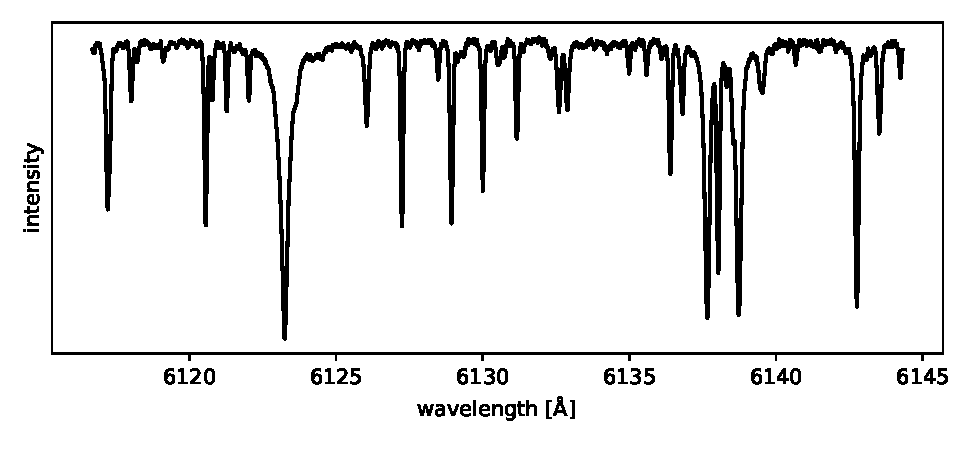
\includegraphics[width=\textwidth]{figures-1/star.pdf}
    \caption[Example of Stellar Absorption Lines -- HD 3651]{Stellar absorption lines within a portion of the spectrum of the star HD 3651.}
    \label{fig:star}
\end{figure}

\begin{figure}
    \centering
    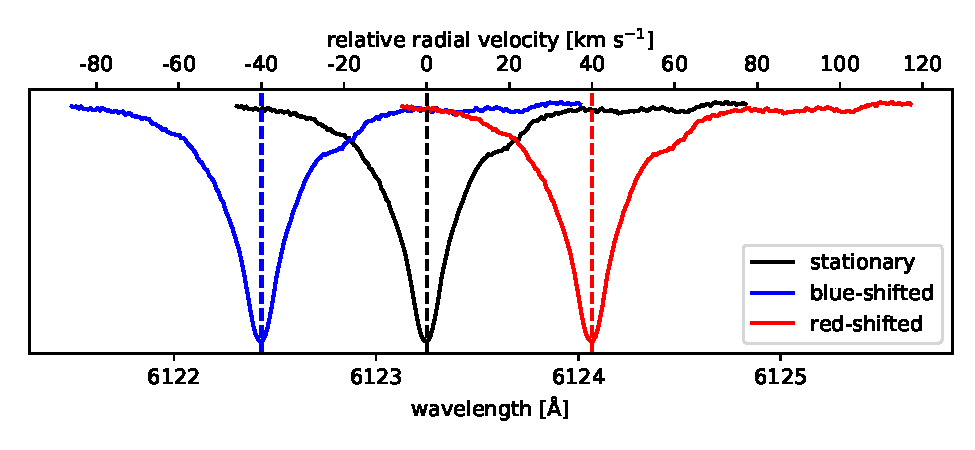
\includegraphics[width=\textwidth]{figures-1/absorption-lines.pdf}
    \caption[Doppler Effect Example -- Change in wavelength of a stellar absorption line]{Change in wavelength for a stellar absorption line caused by both a positive and negative 40\kms radial velocity.}
    \label{fig:absorption-lines}
\end{figure}

Measurement of the Doppler Effect, and therefore RVs, using spectroscopy leverages the existence of atomic absorption lines within the stellar spectra (Figure \ref{fig:star}). As light travels from deep within the hot interior of the star (the stellar continuum, black body radiation that is defined by Wien's Law), some of it is absorbed by the cooler and heavier gas in the outer layers of the star resulting in dimmer gaps across the spectrum. We know at which wavelengths these absorption lines should occur, due to studies in atomic physics and observations of our own Sun, and use them as points of comparison against the stellar spectra we collect with our spectrograph (see Figure \ref{fig:absorption-lines}). As the lines move further away in wavelength from where we expect them to be, the larger the measured RV.

A spectrograph's RV precision is therefore determined by how well it can measure the movement of these stellar absorption lines. There are two primary ways that this precision can be described \citep{fischer_state_2016}: (1) single-measurement precision or (2) long-term velocity scatter. The single-measurement precision states how well the instrument \textit{thinks} it can measure velocities. Resolution, bandwidth, signal-to-noise ratio, and other instrument characteristics are all folded into this value, typically through statistical analysis while calculating the RV. Long-term velocity scatter, on the other hand, requires multiple RVs of the same target star. After a Keplerian model is fit to these RVs, the scatter is found by calculating the average difference (or residual) between the model and the yielded RVs. This second metric is important to include since it may reveal systematic instrument issues unaccounted for in the single-measurement precision.

Finally, consideration needs to be made for the fact that, not only is the observed star moving due to pulls from possible exoplanets but, the Earth is hurtling through space around our own sun at nearly 30,000~\si{\meter\per\second}, much faster than the RV semi-amplitude we are attempting to measure. Therefore, we must also employ a barycentric correction---modification of the wavelengths as if we had measured them from the stationary center of mass of our solar system---to our stellar spectra before making an RV measurement \citep{wright_barycentric_2014}. Briefly, this is done by knowing two critical pieces of information: when ("What time?") and in which direction ("Where are you pointing the telescope?") the observation was made. Then, because the motion of Earth is quite well studied and therefore predictable, we can figure out the velocity the Earth is moving towards or away from the target star at the moment of observation and alter the wavelengths of the spectrum accordingly using Equation \ref{eq:relative-doppler-effect}.

\subsection{Limitations and Alternatives}

Unfortunately, there are some limitations in our ability to measure stellar spectra and these absorption lines consistently over time \citep{lovis_radial_2011}. The first is due to activity in the stellar atmosphere, which we collectively define as stellar noise. Whether it be through p-mode oscillations (large-scale pressure changes), granulation (small cells of convective motion), or cool spots and hot plages (dark and bright surface regions) that rotate with the star, stellar activity can mask itself as false RV signals on the order of 1--5~\si{\meter\per\second} in the motion of the stellar absorption lines. In order to avoid this, users of the RV technique primarily study stars that they know are less noisy or, when possible, observe noisy stars long enough to average over the effects of stellar activity. Otherwise, a large portion of the field of RV spectroscopy is currently trying to find ways of disentangling stellar noise signals from the signals caused by planetary orbits \citep[e.g.][]{davis_insights_2017, dumusque_measuring_2018}.

Another major limitation of the RV technique is caused by Earth's atmosphere in the form of, what is called, telluric contamination. After leaving the star, light travels only through the vacuum of space before finally reaching Earth. At this point, it must pass through an entire atmosphere before reaching the spectrograph, picking up new absorption lines from gases such as molecular oxygen and water vapor. These telluric lines can overlap heavily with stellar absorption lines and, most importantly, they do not move with the radial velocity of the star. Rather, telluric lines need to be modeled and divided out or simply masked and avoided in RV measurement. Near-infrared spectrographs are hit hardest by telluric contamination due to the high opacity of the Earth's atmosphere (primarily water) in these wavelength regions.

Further limitations on RV measurement come from the instrumentation and spectrograph design. Throughput of light coupled from the telescope to the spectrograph is crucial to maximize. Less light from a single observation leads directly to lower RV precision, but we would prefer to not spend an entire night looking at a single target star to collect a high signal-to-noise spectrum. Moreover, this throughput tends to be inversely correlated with the resolution of the instrument, meaning careful consideration needs to be made to find a compromise between designed signal-to-noise and resolution \citep{davis_insights_2017}. Also, consistency in the path of light as it travels through the spectrograph enables repeatable observations night after night. Factors such as temperature and pressure must be held nearly constant to avoid significantly altering the optical path and external vibrations must be absolutely mitigated to prevent movement in the physical structure of the spectrograph optics. All told, the systematic effects of the instrument need to be significantly smaller than the amplitude of planetary signals, or otherwise carefully characterized, in order to have a chance at precision detection. This is especially true when trying to disentangle all three possible sources of motion: planets, stellar noise, and the instrument itself.

There have been numerous other methods of detecting and characterizing exoplanets, helping to fill out more possibilities of discovery as well as supplementing measurements made by the RV technique \citep{fischer_exoplanet_2014}. In particular, the transit method---whereby a precision brightness-measuring instrument looks for exoplanets passing directly between its host star and the Earth, briefly dimming the stellar intensity---can provide information about exoplanet radii, enabling planet density approximations when combined with mass estimates from the RV technique. The two major transit method satellite missions---Kepler \citep{borucki_kepler_2010}, along with its extension mission K2 \citep{howell_k2_2014}, and TESS \citep{ricker_transiting_2014}---are also providing thousands of exoplanet candidates with corresponding orbital periods, enabling better determination of observing strategies for the RV technique. Other exoplanet-detecting techniques include direct imaging (measuring the light reflected off an exoplanet from its host star after blocking light from the star with a coronagraph), microlensing (measuring the general relativistic bending of light due to the gravity of an exoplanet), and astrometry (measuring non-radial stellar positions over time).

\section{The State of the Field}

The history of exoplanet detection with the RV technique can be traced back through the various spectrographs used to make these measurements. Figure \ref{fig:rv-exoplanets}, a compilation of exoplanets discovered using the RV technique by their RV semi-amplitude, clearly shows the progress made so far and the work we have ahead of us. From 1995 to 2010, there was steady improvement in measurement precision, with the minimum RV semi-amplitudes of planets discovered with the RV technique steadily decreasing from 100~\si{\meter\per\second} to below 1~\si{\meter\per\second} within this period. Over the past ten years, however, highest precision discoveries have halted at about the 0.5--1.0~\si{\meter\per\second} level, likely due to stellar activity being difficult to distinguish from planet-induced RVs at this instrumental precision. The role of those currently in RV instrumentation, myself included, is to provide the tools necessary to break past this barrier.

\begin{figure}
    \centering
    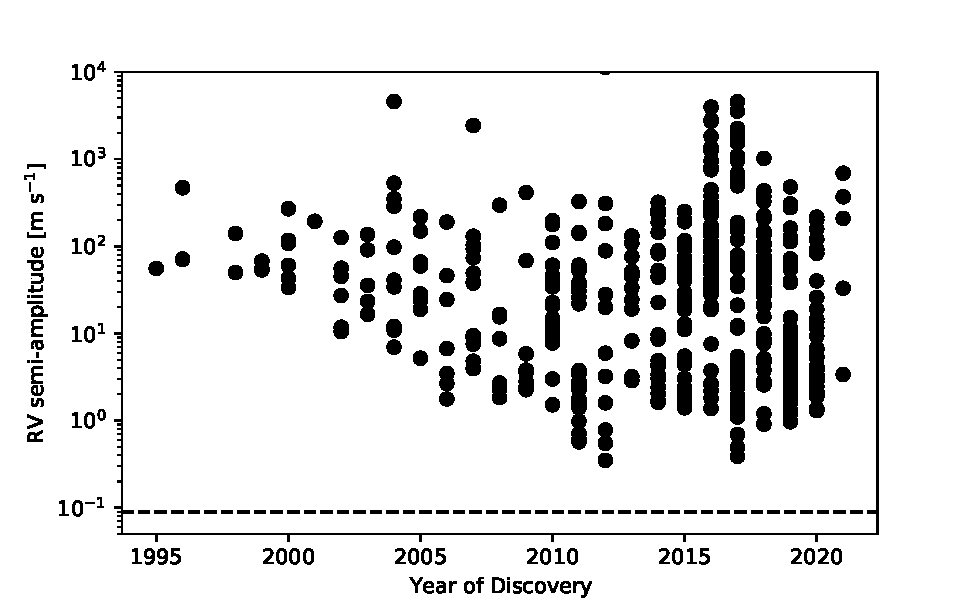
\includegraphics[width=\textwidth]{figures-1/rv-exoplanets.pdf}
    \caption[Radial-velocity Technique Timeline -- Exoplanet discoveries by year and semi-amplitude]{Confirmed exoplanets by year of discovery and measured RV semi-amplitude (data compiled using \url{exoplanet.eu} on 1/31/2021). The horizontal dashed line indicates the RV semi-amplitude of Earth.}
    \label{fig:rv-exoplanets}
\end{figure}

Table \ref{tab:spectrographs} lists just a handful of the many instruments---along with their designed resolution, bandwidth, and single-measurement RV precision---that have made measurement with the RV technique possible. More comprehensive lists can be found in \citet{fischer_state_2016} and \citet{wright_third_2017}. I have loosely grouped them into categories based on my own perceived ``eras'' of RV planet searches and briefly describe them here.

\begin{table}
    \centering
    \small
    \begin{tabular}{lcccc}
        \hline
        \hline
        Spectrograph & Year & Resolution & Bandwidth (nm) & SMP (~\si{\meter\per\second}) \\
        \hline
        Hamilton & 1987 & 50,000 & 390-800 & 3.0 \\
        ELODIE & 1993 & 42,000 & 390--680 & 10.0 \\
        HIRES & 1996 & 55,000 & 364--800 & $3.0\rightarrow1.5$ \\
        Tull & 1998 & 60,000 & 345--980 & 5.0 \\
        HRS & 2001 & 60,000 & 408--784 & 3.0 \\
        \hline
        HARPS & 2003 & 115,000 & 380--690 & 0.8 \\
        SOPHIE & 2006 & 75,000 & 387--694 & 1.1 \\
        PFS & 2010 & 76,000 & 390--670 & 1.2 \\
        CHIRON & 2011 & 90,000 & 440--650 & 1.0 \\
        HARPS-N & 2012 & 115,000 & 380--690 & 0.8 \\
        PARAS & 2012 & 67,000 & 380--690 & 1.0 \\
        APF+Levy & 2013 & 100,000 & 374--950 & 1.0 \\
        \hline
        MINERVA & 2016 & 75,000 & 480--690 & 0.9 \\
        CARMENES & 2016 & 90,000 & 520--1710 & 1.0 \\
        HPF & 2017 & 50,000 & 970--1810 & 1.0 \\
        MINERVA-Red & 2018 & 75,000 & 820--920 & 1.0 \\
        ESPRESSO & 2018 & 134,000 & 380--780 & 0.1 \\
        EXPRES & 2018 & 137,500 & 380--840 & 0.3 \\
        MAROON-X & 2019 & 80,000 & 500--900 & 1.0 \\
        PARVI & 2019 & 100,000 & 1250--1800 & 0.3 \\
        iLocater & 2019 & $>$150,000 & 971--1270 & 0.7 \\
        NIRPS & 2019 & 100,000 & 970--1810 & $<$1.0 \\
        NEID & 2020 & 100,000 & 380--1000 & 0.3 \\
        KPF & 2021 & 85,000 & 440--850 & 0.3 \\
        G-CLEF & 2023 & 100,000 & 350--950 & 0.1 \\
        \hline
    \end{tabular}
    \caption[History of radial-velocity spectrographs]{Past, current, and future RV spectrographs with tested or predicted metrics \citep{fischer_state_2016, wright_third_2017}.}
    \label{tab:spectrographs}
\end{table}

The detection of 51 Pegasi b was accomplished with the ELODIE spectrograph \citep{baranne_elodie_1996}, which actually had lower resolution and single-measurement precision than other astronomical spectrographs at the time. The Hamilton spectrograph \citep{vogt_lick_1987} at Lick Observatory, rather, had been searching for exoplanets since 1987 and was used to great effect, eventually with over 300 target stars \citep{fischer_planetary_1999}, until its decommissioning in 2011. The true workhorse of this era (and even some to this day) is the High-Resolution \'Echelle Spectrograph \citep[HIRES;][]{vogt_hires_1994} on the Keck Observatory 10~m telescope, observing more than 4000 target stars and steadily improving measurement precision through instrument upgrades up to 1.5~\si{\meter\per\second}. Other spectrographs from this period include the High Resolution Spectrometer \citep[HRS;][]{tull_high-resolution_1998} at the Hobby-Eberly Telescope and the Tull Spectrograph \citep{tull_high-resolution_1995} at McDonald Observatory.

Then, in 2003, the High-Accuracy Radial velocity Planetary Searcher spectrograph \citep[HARPS;][]{pepe_harps_2002, mayor_setting_2003} at the La Silla 3.6~m telescope in Chile set the new standard for RV spectroscopy. It was the first such instrument primarily designed to search for exoplanets and therefore included superior temperature, pressure, and vibration stability. This enabled an almost doubling of previous-generation resolution and an improvement to less than 1.0~\si{\meter\per\second} precision, both significant achievements at the time. HARPS thus ushered in a wave of exoplanet discoveries, especially super-Earth- and Neptune-mass planets around solar-type stars \citep{pepe_harps_2011}, with over 2000 target stars. Over the next decade, older RV spectrographs began to be upgraded or replaced to meet this new standard: SOPHIE \citep{perruchot_sophie_2008} replaced ELODIE while the Automated Planet Finder with the Levy spectrograph \citep[APF+Levy;][]{vogt_apflick_2014} took the place of Hamilton. Also, a few new-concept spectrographs came online, including CHIRON \citep{tokovinin_chironfiber_2013}, the PRL Advanced Radial-velocity Abu-sky Search spectrograph \citep[PARAS;][]{chakraborty_first_2010, chakraborty_prl_2014} and the Planet Finder Spectrograph \citep[PFS;][]{crane_carnegie_2006}. The success of HARPS also prompted a near copy to be built in the northern hemisphere in 2012 \citep[HARPS-N;][]{cosentino_harps-n_2014}.

Now, we are in the era of the ``next-generation'' of RV spectroscopy corresponding to an explosion of new high-resolution spectrographs coming online within the last five years. This large diversity RV spectrographs has enabled incredible innovation. Many new spectrographs---such as CARMENES \citep{quirrenbach_carmenes_2016}, HPF \citep{mahadevan_habitable-zone_2014}, NIRPS \citep{wildi_nirps_2017}, and PARVI \citep{gibson_characterization_2020}---are beginning to explore the near-infrared, and therefore more M-type stars, to search for planets. Spectrographs like ESPRESSO \citep{pepe_espresso_2013}, EXPRES \citep{jurgenson_expres_2016}, and NEID \citep{schwab_design_2016}, as well as future designs such as KPF \citep{gibson_kpf_2016} and G-CLEF \citep{szentgyorgyi_gmt-consortium_2016}, on the other hand, are pushing the boundaries of visible-band spectroscopy through higher resolution, greater bandwidth, and extreme measures for environmental stability. We even have projects like iLocater \citep{crepp_ilocater_2016} that are trying to achieve extremely high resolution in the near-infrared. This truly is an exciting time to be an exoplanet hunter with the RV technique as there are simply so many avenues for possibility.

\section{The EXtreme PREcision Spectrograph} \label{intro:expres}

Nearly all of the work presented in this thesis was completed in support of the EXtreme PREcision Spectrograph \citep[EXPRES;][]{jurgenson_expres_2016, blackman_performance_2020, petersburg_extreme-precision_2020}, a high-resolution RV spectrograph commissioned at the Lowell Discovery Telescope outside Happy Jack, Arizona, in 2018. EXPRES was built as part of the 100-Earths Survey, a collaboration between the Yale University and Lowell Observatory, with the express goal of finding 100 Earth-like planets within the next decade. Considering this requires RV measurement at the 0.1~\si{\meter\per\second} level, the designing, commissioning, and maintenance of EXPRES has proven to be a scientific and engineering feat since it was first conceived in 2014. This has involved everything from advanced optical fiber and laser technology, to precisely tuned environmental stability systems, to the development and implementation of new software to analyze data.

Therefore, in this section, I will be using EXPRES as a guide to introduce the physical and virtual mechanisms required make such precise measurements as the 0.1~\si{\meter\per\second} wobble of a star. Naturally, the design decisions that went into EXPRES were built upon the strong pedigree of the RV community introduced in the previous section. Some of our decisions may differ from those of our contemporaries, but I try to address concerns as I have seen them. In the case of EXPRES, instrument design for RV spectroscopy can be split into four critical areas: (1) the optical fiber infrastructure, (2) the \'echelle spectrograph, (3) wavelength calibration sources, and (4) the data extraction software. I introduce these areas here to motivate the work completed in this thesis.

\subsection{Optical Fiber Infrastructure} \label{intro:optics:fiber}

The first consideration for an RV spectrograph is determining how to couple light from a telescope into the instrument. Traditionally, instruments are attached right at a focus of the telescope, as is the case with many early RV spectrographs including HIRES, HRS, and Hamilton. However, considering the telescope moves constantly throughout the night to track target stars and is typically exposed to outside air temperature changes, this can cause problems with vibrational and thermal stability.

Instead, many RV spectrographs, including EXPRES, are coupled via optical fiber to the telescope. Optical fibers are long (meters to kilometers) thin (micrometers) tubes of glass that are able to transmit light from one end to the other, typically with high throughput across a wide range of wavelengths. In principle, optical fibers propagate light due to a difference in the refractive index---a property ($n$) that determines the speed light moves through the material ($v=c/n$)---of the two concentric glass cylinders that make up the length of the fiber: the inner core and the outer cladding. When light enters the core at an angle and reaches the surface boundary at the cladding, rather than being transmitted into the cladding, the light reflects off the surface and continues traveling down the core, effectively bouncing its way from one end of the fiber to the other. This enables a great deal of flexibility in moving light from one place to another, since optical fibers can be bent around corners and precisely attached to other optical systems at either end.

Therefore, the use of optical fibers provides a great boon to RV spectroscopy. The spectrograph can be placed in a separate, possibly temperature-controlled and vibrationally-isolated, room near to the telescope (rather than on the telescope itself) with little loss to throughput. Optical fibers also provide spatial scrambling to stellar light, meaning input variations of the light---such as poor telescope guiding or changes in atmospheric density---are smoothed over before illumination of the spectrograph optics \citep{hunter_scrambling_1992}. This effect can also be amplified through the use of a fiber-coupled double scrambler \citep{halverson_efficient_2015, spronck_fiber_2015} and a non-circular fiber cross-section \citep{chazelas_new_2010, spronck_use_2012, plavchan_precision_2013}. Finally, optical fibers enable many possibilities for alternative light sources, beyond the telescope, to enter the spectrograph. In the case of EXPRES, this involves an entire ``fiber architecture'' (Figure \ref{fig:expres-fibers}) that includes multiple wavelength calibration sources (see Section \ref{intro:wvln_cal}), a flat-field calibration source (through two different sizes of fiber), and even an entirely separate telescope that observes the Sun \citep{blackman_performance_2020}.

\begin{figure}
    \centering
    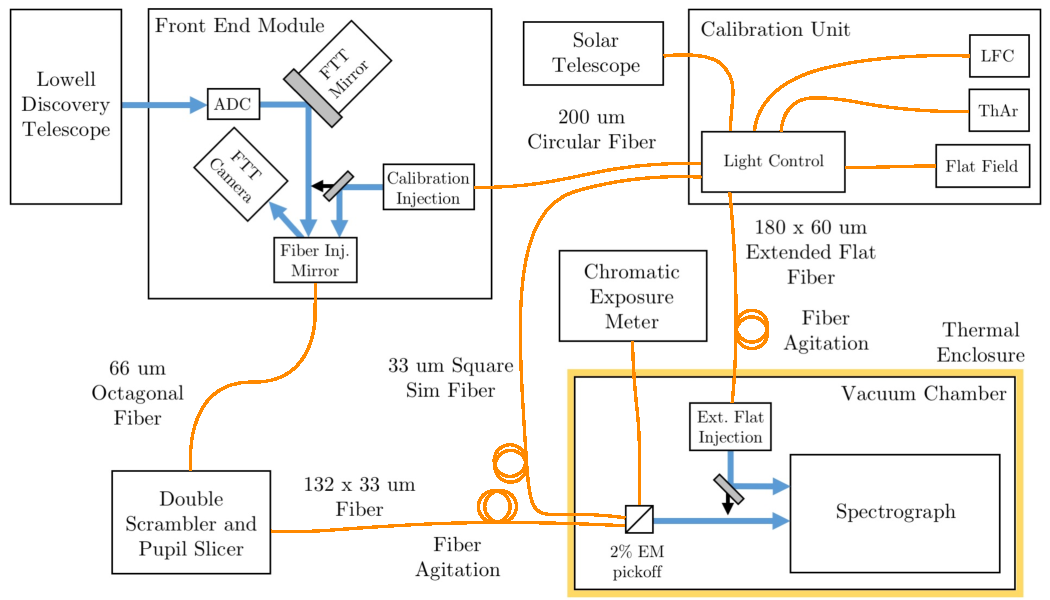
\includegraphics[width=\textwidth]{figures-1/expres_schematic_fibersV3.pdf}
    \caption[The EXPRES Fiber Architecture]{The EXPRES fiber architecture, reprinted from \citet{blackman_performance_2020}.}
    \label{fig:expres-fibers}
\end{figure}

There are, however, a few downsides to the use of optical fibers. To understand them, I will first introduce the ideas of focal ratio and numerical aperture. Light diverging from or converging to a single focus (such as is done by the cornea onto the retina of the human eye) does so in the shape of a cone, where the focus sits at the tip and the focusing optic (lens or mirror) sits at the base. The focal ratio (or $f/\#$) is the ratio between the height of this cone and the diameter of the base; a ``fatter'' cone means a lower focal ratio. The numerical aperture of an optical fiber---determined by the relative indices of refraction between the core and cladding ($\mathrm{NA}=\sqrt{n_{core}^2-n_{clad}^2}$)---then defines the minimum focal ratio accepted by the input ($f/\#_{min} \approx \frac{1}{2\mathrm{NA}}$). If light enters the fiber core at too steep an angle, it will not reflect off the cladding but rather dissipate out of the fiber.

Most optical fibers exhibit some form of focal ratio degradation (FRD), where light injected at a certain focal ratio is then output at a slightly lower focal ratio closer to the numerical aperture. FRD is exacerbated by tight bends and especially cracks in the fiber \citep{ramsey_focal_1988}. This means the focal ratio of the telescope should not exceed the numerical aperture of the optical fiber and the fibers need to be vetted and characterized for FRD to understand how the cone of light will change before entering the spectrograph. The spectrograph subsequently needs to be designed such that it will accept as much of the output cone of light as possible. The other major issue with optical fibers, modal noise, is more comprehensively introduced and rectified in Chapter \ref{chapter:modal-noise}.

\subsection{The \'Echelle Spectrograph} \label{intro:optics:echelle}

\begin{figure}
    \centering
    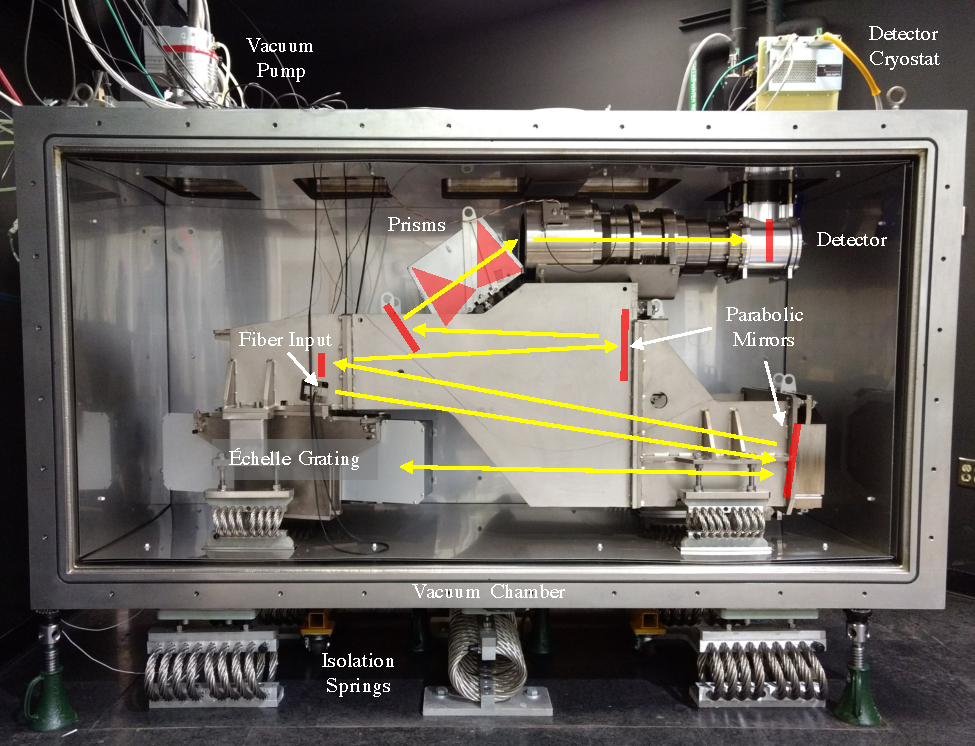
\includegraphics[width=\textwidth]{figures-1/expres.pdf}
    \caption[The EXPRES \'Echelle Spectrograph and Optical Path]{Photograph of the EXPRES \'echelle spectrograph with an overlayed optical path and labels for the various optical component, also shown overlayed in red.}
    \label{fig:expres}
\end{figure}

Once light is coupled from the telescope, nearly all RV spectrographs follow a similar optical path to the one shown in Figure \ref{fig:expres} for EXPRES. This type of instrument is known as an \'echelle spectrograph. Diverging light from the input is collimated---made parallel or directed, like light from a laser pointer---by a parabolic mirror towards the \'echelle grating. An \'echelle grating serves a similar function to the prism in my example earlier, separating the light into its various constituent wavelengths spatially. However, it is not a single continuous spectrum. Rather, an \'echelle grating exploits the diffraction equation ($d \sin{\theta} = m \lambda$) to reflect multiple shorter spans of spectra that happen to be spatially overlayed with each other. Consider two separate sets of grating orders ($m$) and wavelengths: ($m_1=100$, $\lambda_1=500~\mathrm{nm}$) and ($m_2=150$, $\lambda_2=400~\mathrm{nm}$). Each of these pairs yield the same $d\sin{\lambda}$ (or $m_1\lambda_1 = m_2\lambda_2$) meaning they are reflected at the exact same angle by the \'echelle grating. The EXPRES \'echelle grating is designed to maximally reflect overlapping segments of grating orders 84 to 160 right back at the first parabolic mirror.

After the \'echelle grating, the light is then focused near a small optical correcting mirror, which subsequently reflects the light back to another parabolic mirror. The re-collimated light is then reflected again using a simple flat mirror through a pair of cross-dispersing prisms. These prisms vertically separate the overlapping orders produced by the \'echelle grating, enabling us to differentiate between them spatially. These prisms are called ``cross-dispersers'' because they diffract the light perpendicularly to the \'echelle grating ``disperser.'' After traveling through the prisms, the light is finally focused onto the spectrograph's detector, yielding the \'echellogram shown in Figure \ref{fig:expres-format}. Just like the orientation of EXPRES, the horizontal dimension of this image is known as the dispersion direction and the vertical dimension is known as the cross-dispersion direction. The smoothly varying brightness of the continuum across each order is known as the blaze function, an inherent property based on the reflection efficiency of the \'echelle grating.

\begin{figure}
    \centering
    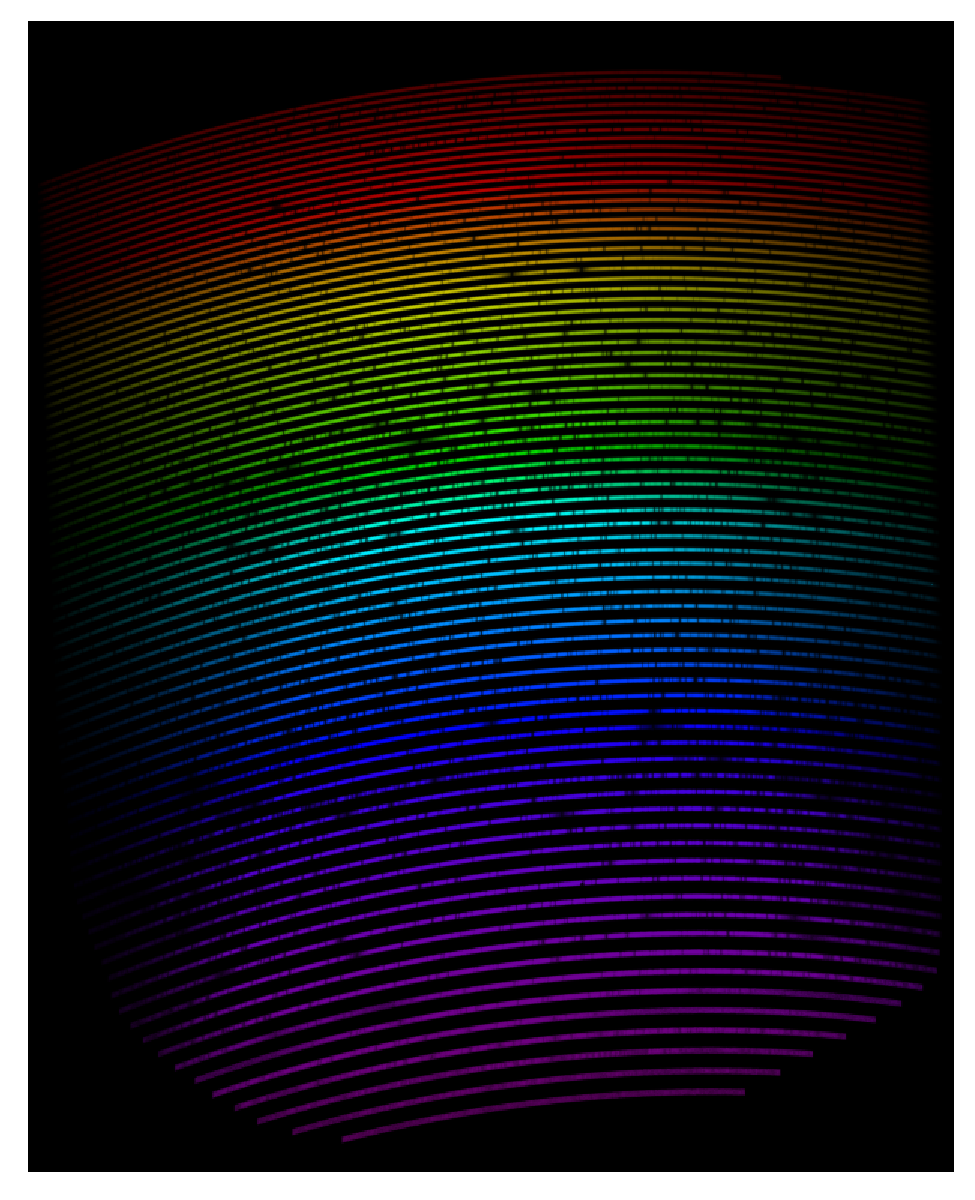
\includegraphics[width=\textwidth]{figures-1/expres-format.pdf}
    \caption[The EXPRES \'Echelleogram]{The EXPRES true-color \'echellogram for an observation of the star HD 3651 taken on October 24, 2020. Each distinct arc is a unique \'echelle grating order. Wavelength increases from left to right across each order and from bottom to top between orders. The peak brightness of each order is artificially normalized to match the others in this image.}
    \label{fig:expres-format}
\end{figure}

The EXPRES detector (that produced Figure \ref{fig:expres-format}) is a Charge-Coupled Device (CCD) that converts photons (particles of light) into electrons (particles of electric charge) within a large number of discrete pixels arranged as a two-dimensional array. The rate of success with which each pixel can make this conversion is called its quantum efficiency. The CCD, after a set exposure time, then transfers and amplifies these electrons through a series of read-out electronics to convert them into a digital signal for processing by a computer. The conversion ratio between this digital value and the true number of counted electrons is called the gain. There are two important sources of noise during this process: photon noise and read noise. Photon noise is caused by the quantized nature of light: only an integer number of photons can hit any given pixel. Therefore, random fluctuations in brightness are predicted by Poisson statistics, meaning the expected standard deviation of $N$ photons hitting a given pixel is $\sigma_\gamma=\sqrt{N}$. Read noise is rather an inherent property of each CCD pixel. As the photon-induced electrons (or photo-electrons) are read out, there is some constant scatter to the values, whose standard deviation is defined as the read noise ($\sigma_r$). These two terms are typically added in quadrature ($\sigma=\sqrt{\sigma_\gamma^2 + \sigma_r^2}$) to yield a complete noise model for each CCD pixel. Ideally, CCDs are developed with maximum quantum efficiency and minimum read noise.

Figure \ref{fig:expres} also reveals some of the environmental stability measures taken by EXPRES \citep{jurgenson_expres_2016}. The entire optical bench is built within a large vacuum chamber (meaning we are normally not able to see it) to maintain an extremely low and stable pressure ($1\times 10^{-7} \pm 2\times 10^{-8}$~torr) as well as less than 0.075~\si{\kelvin} per day drifts in temperature \citep{blackman_performance_2020}. The optical bench itself is also constructed from Invar, a nickel-iron alloy that flexes very little with changing temperature. Along the bottom are two sets of springs that vibrationally isolate the spectrograph from the slab it is sitting on, which itself is physically isolated from the rest of the telescope building foundation. Finally, the EXPRES detector is super-cooled and temperature controlled with an independent cryostat to minimize thermal effects on the CCD.

\subsection{Wavelength Calibration} \label{intro:wvln_cal}

In order to extract stellar spectra, RV spectrographs use the spectra of well-characterized and stable light sources as a simultaneous or observation-bracketing reference on the spectrograph camera. These can be thought of as the ``yardsticks'' of RV measurement. Historically, thorium argon (ThAr) lamps and iodine reference cells have been used to calibrate RV spectrographs since their spectral properties are well understood and their bandwidth covers most of the visible spectrum. However, both of these light sources have inherent issues that limit RV measurements to approximately \SI{1}{\meter\per\second} precision. ThAr emission lines are broad, saturated, and irregularly spaced, meaning some wavelength regions are less well calibrated than others. The iodine technique---which instead applies known absorption wavelengths directly on the stellar spectrum---masks the subtle indicators of stellar activity and introduces complexity to the RV measurement process \citep{spronck_fiber_2015}. Furthermore, the cells themselves may not have long term mechanical stability \citep{fischer_twenty-five_2014}.

More recently, RV spectrographs have employed frequency combs (FCs), synthesized spectra containing sharp peaks of intensity at equally spaced frequencies, with the intention of better stability and therefore precision in their wavelength calibration. Ideally, the lines of a FC are non-overlapping and located at precisely determined wavelengths with flat intensity, to avoid over- or under-saturating pixels on the spectrograph detector. The FC must also have the proper free spectral range (FSR, frequency separation of comb lines) across the entire bandwidth of the spectrograph so that the detector can resolve each peak (more than \SI{10}{\giga\hertz}) and calibrate a sufficient number of stellar frequencies (less than \SI{40}{\giga\hertz}). Also, the zero-point frequency offset ($f_0$) and FSR should not drift over both short (seconds) and long (months) time scales. Most FC devices have been developed for the near-infrared, due to the proliferation of telecom interest around \SI{1550}{\nano\meter}, and this has been sufficient for detecting exoplanets around M-type stars \citep{fischer_state_2016}. However, to address planetary system statistics for late F, G, and early K type stars, the wavelength range will need to stretch through the visible to better calibrate many more absorption lines. It is especially important to reach the Calcium H \& K lines located below 400\si{\nano\meter} that contain indicators of stellar activity \citep{isaacson_chromospheric_2010, lovis_harps_2011}.

A relatively cheap way to produce a broadband optical FC is using a tunable Fabry-P\'erot etalon, a resonant cavity that employs feedback to correct for drifts in the distance between the two reflective surfaces. They do not offer an inherent $f_0$ calibration, however, and must be referenced against a separate stable source for bootstrapped calibration \citep{mccracken_single-lock_2014, sturmer_rubidium-traced_2017} meaning the system cannot be self-contained. Therefore, fixed-length Fabry-P\'erot etalons were developed to mitigate this issue. However, \citet{reiners_laser-lock_2014} and \citet{wildi_passive_2012} have shown that the set distance between the two reflective surfaces still drifts unpredictably, especially over long time scales, thereby continuing to limit spectrograph precision to only $\sim$\SI{1}{\meter\per\second}.

Menlo Systems has built perhaps the most advanced wavelength calibrator for visible RV spectroscopy, a laser FC that reaches 1\si{\centi\meter\per\second} RV precision \citep{probst_laser_2014}. This FC pulses a femtosecond mode-locked laser to produce high finesse lines and an extremely stable FSR. Unfortunately, these lines are too tightly spaced for RV spectrographs, therefore the system must use line-by-line spectral filtering with multiple tunable Fabry-P\'erot cavities to suppress most of the produced frequencies. There are consequently some critical limitations to this device: complexity, cost, and limited bandwidth. The Menlo FC requires a continuing service contract to properly maintain it and thus has not yet reach true ``turn-key'' status. Also, this technology costs approximately \$1,000,000---a prohibitive price point for smaller RV projects---and is extremely bulky, limiting its use to larger ground-based spectrographs. Furthermore, the system is still blue-limited to no less than 450\si{\nano\meter} thereby excluding the critical Calcium H \& K lines below 400\si{\nano\meter}.

A promising and growing field of astro-comb development includes electro-optic modulation combs and chip-based waveguide technologies \citep[e.g.][]{carlson_ultrafast_2017, yi_demonstration_2016, obrzud_broadband_2018, obrzud_visible_2019}. These devices offer ease-of-use along with a much more affordable price point, since electro-optic combs can be built using primarily off-the-shelf components while waveguides can be fabricated and tuned in-house to meet the needs of the instrument. These technologies are the focus of my work in Chapter \ref{chapter:astro-comb}, therefore, I provide further introduction to them there.

Emission line wavelength calibration sources have another important function for the instrument: point-spread-function characterization. Since an \'echelle spectrograph converts spectral information into spatial information, a spectral point source (i.e. a single wavelength laser) would ideally be mapped as a physical point source on the spectrograph's detector. However, within any optical re-imaging system, light is not perfectly translated from input to output. Rather, the light undergoes optical aberrations modifying it as it is reflected and diffracted throughout the system and, importantly, these effects are typically wavelength dependent. Therefore, shining a single wavelength laser into a spectrograph reveals exactly the optical aberrations, or point spread function, of the instrument at that wavelength. Emission line wavelength calibration sources are simply a collection of hundreds or thousands of such single wavelength lasers, thus they can be used to map the point spread function of a spectrograph across its entire spectral format.

EXPRES uses a Menlo LFC primed by a ThAr lamp to complete its nightly wavelength calibrations. The principles of this process are shown in Figure \ref{fig:calibration}. The wavelengths of ThAr emission lines are easily identifiable using data from previously collected ThAr atlases \citep{palmer_atlas_1983, redman_spectrum_2014}. These lines then provide a close guess for the wavelengths of some LFC lines which can subsequently all be identified using the LFC's known FSR and $f_0$. These wavelengths are then interpolated to match the grid of spectral bins of the provided spectrum. Additionally, ThAr lines outside the bandwidth of the LFC are used to provide the wavelengths in these spectral regions. Further specifications for this process for EXPRES can be found in Chapter \ref{chapter:pipeline}.

\begin{figure}
    \centering
    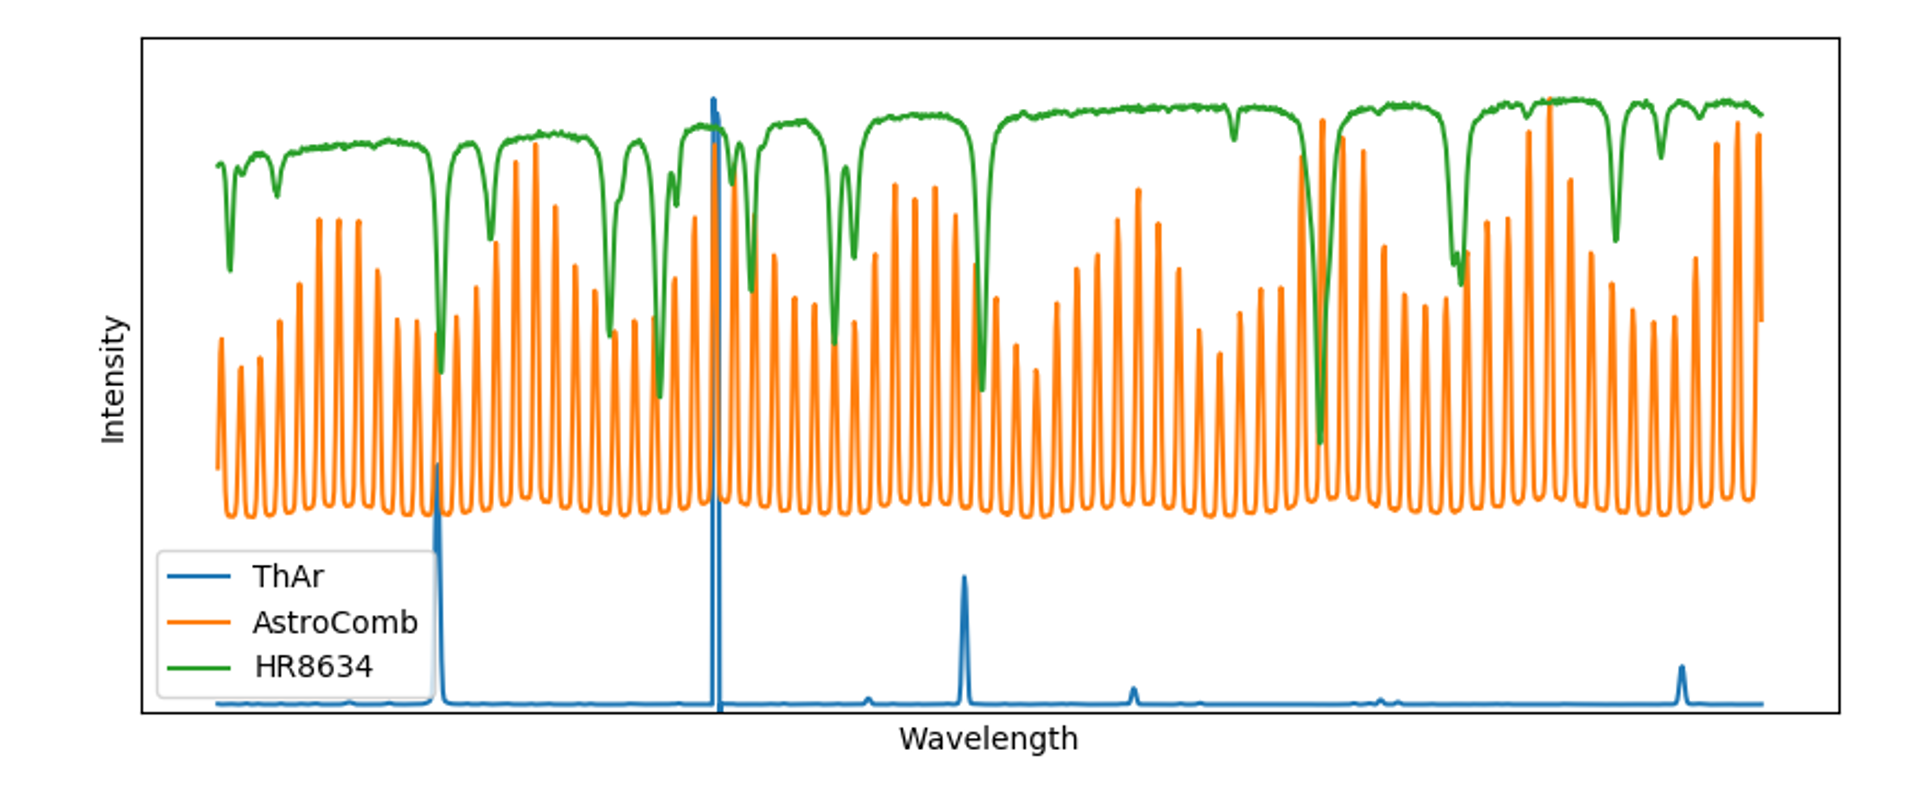
\includegraphics[width=\textwidth]{figures-1/calibration.png}
    \caption[EXPRES Wavelength Calibration]{Three stages of wavelength calibration for EXPRES. ThAr lines are used as a primer for the LFC (AstroComb) lines which are finally used to generate wavelengths for the stellar spectrum (here a section of HR 8634).}
    \label{fig:calibration}
\end{figure}

Finally, consideration needs to be made as to \textit{when} wavelength calibrations are made as part of the observation strategy. Namely, the decision between simultaneous calibrations---measuring the wavelength calibrator at the same time as the star through a separate fiber---and bracketed calibrations---using the same fiber but alternating between stellar and calibration observations. Simultaneous calibrations have two inherent downsides: (1) a requirement to tailor the brightness of the calibrating light source to match signal-to-noise over various length of science observations (i.e. brighter vs. dimmer stars) and (2) systematic changes in the optical system may not perfectly correlate between separate fibers, meaning extra analysis is necessary to translate wavelength solutions generated by the simultaneous calibration light path to the science light path. Therefore, EXPRES uses bracketed calibrations in order to more consistently control the brightness of its laser frequency comb (which can reach a sufficient signal-to-noise level within only 10 seconds) and to calibrate the instrument using the same optical path and detector pixels as science observations. As demonstrated in Chapter \ref{chapter:pipeline}, various methods of interpolation are more than sufficient to then project these bracketed wavelength solutions to midpoint time of intermediate observations.

\subsection{Data Extraction} \label{intro:extraction}

The final step of completing an RV spectrograph is in developing code for data extraction: taking raw pixel data from the instrument's detector, converting it into a wavelength-calibrated barycentric-corrected spectrum, and using it to calculate the RV of the given observation. Unfortunately, the raw data of EXPRES is not as nice as in Figure \ref{fig:expres-format}, but instead looks like Figure \ref{fig:expres-raw}. The EXPRES CCD is split into 16 distinct regions (four of which we omit to save storage space) which each have their own overscan regions (virtual pixels that reveal fundamental properties of the read-out electronics) and gain. The first step of extraction, which I call ``reduction'', involves combining these separate regions while correcting (QE, gain, dark counts, bias) or characterizing (photon noise, read noise) inherent properties of the data.

\begin{figure}
    \centering
    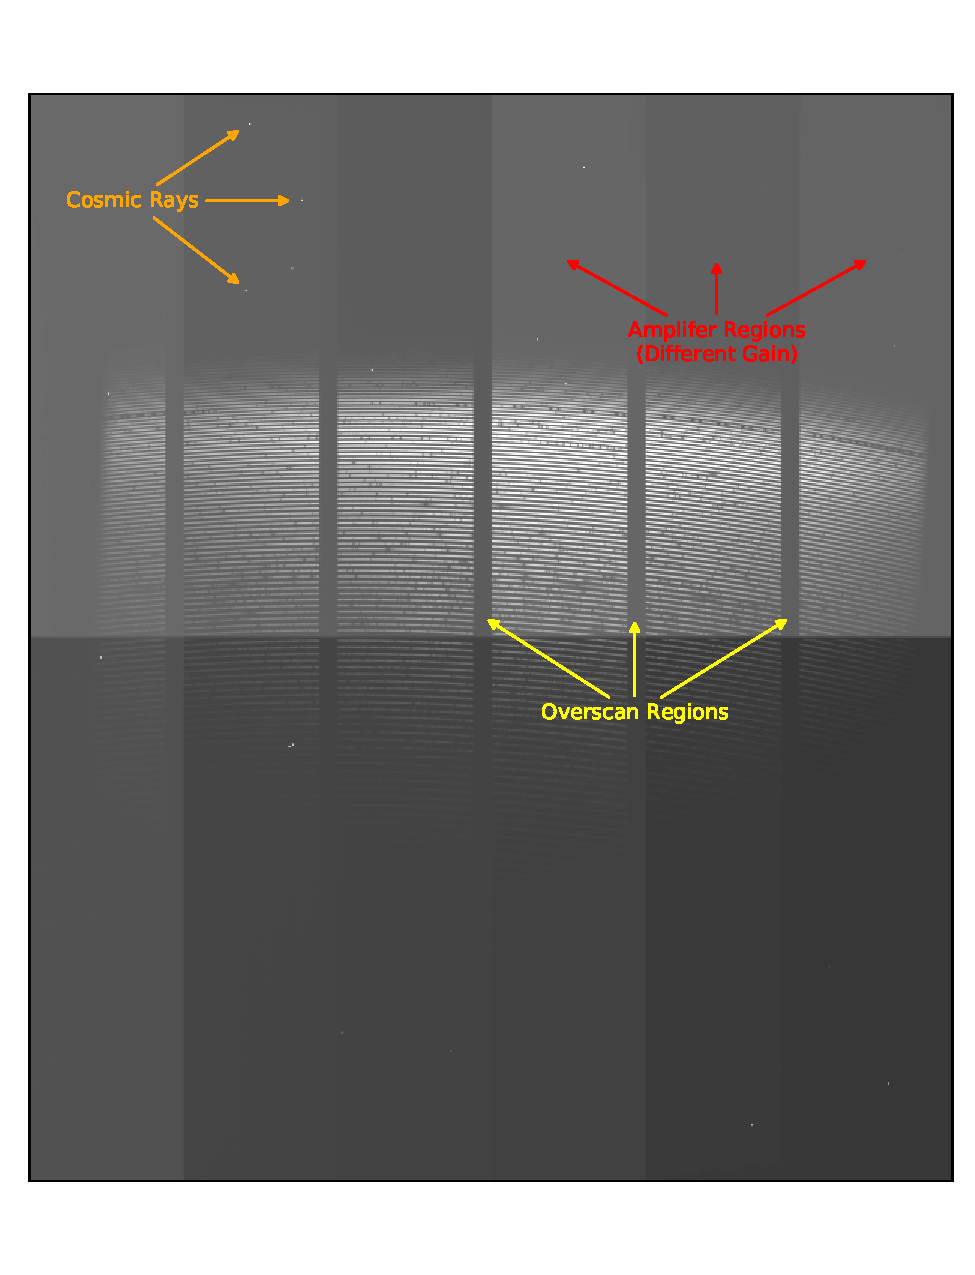
\includegraphics[width=\textwidth]{figures-1/expres-raw.pdf}
    \caption[EXPRES Raw CCD Frame]{Raw frame from the EXPRES detector showing the same observation as in Figure \ref{fig:expres-format}. Only 12 of the 16 CCD amplifier regions are saved to minimize virtual storage usage. Examples of cosmic rays, amplifier regions, and overscan regions are labeled.}
    \label{fig:expres-raw}
\end{figure}

After reduction, the two-dimensional intensity data contained within the 86 separate \'echelle orders is converted into a one-dimensional spectrum. Historically, there have been three methods of spectral extraction developed for RV spectrographs. Boxcar extraction involves simply summing up counts column-by-column along each order. Optimal extraction takes this a step further by developing an expected model for the cross-sectional shape of each order and fitting only a scaling factor to each column, enabling improved signal-to-noise performance and cosmic-ray rejection \citep{horne_optimal_1986}. Finally, spectro-perfectionism has provided a framework for expanding this model into a second dimension, enabling maximum information transfer from CCD to spectrum \citep{bolton_spectro-perfectionism_2009}. Further introduction to optimal extraction and spectro-perfectionism are provided in Chapters \ref{chapter:pipeline} and \ref{chapter:pipeline2} respectively. Introductions to methods for wavelength calibration, barycentric correction, and telluric modeling are also all provided in Chapter \ref{chapter:pipeline}.

Finally, we reach the stage of calculating the RV for each stellar observation. Cross-correlation \citep{baranne_coravel_1979}, taking a delta-function model of the known stellar lines and convolving this against the spectrum to find a maximum overlap point, has been extremely popular and successful at measuring RVs for a wide variety of instruments \citep[e.g.][]{freudling_automated_2013, brahm_ceres_2017, modigliani_espresso_2019}. More recently, however, further exploration has gone into forward modeling techniques---using generated templates of stellar spectra as models for least-squares fitting of an offset velocity \citep[e.g.][]{zechmeister_spectrum_2018, rajpaul_robust_2020}. An important part of either of these processes lies in the identification of stellar activity indicators within the spectrum \citep[e.g.][]{davis_insights_2017, dumusque_measuring_2018}, in order to avoid/mitigate potentially problematic stellar lines or to provide a systematically-corrected offset to the calculated RV. With a series of RV measurements for a given stellar target in hand, we can finally fit the stellar orbit using our Keplerian RV model (Equation \ref{eq:kepler-rv}) and determine characteristics about newly discovered exoplanets.

\section{Thesis Outline} \label{intro:structure}

In this thesis, I present the design and implementation of multiple novel methods---within instrumentation and data extraction---that have demonstrated significant improvement to many aspects of fiber-fed RV \'echelle spectroscopy. The ultimate goal of this entire body of work is to help push exoplanet detection with the RV technique below 0.1~\si{\meter\per\second} Doppler precision, enabling the discovery of Earth-like exoplanets.

Chapter \ref{chapter:modal-noise} describes investigations into the inherent properties of optical fiber modal noise and conclusions about how best to mitigate this potentially devastating noise source. Chapter \ref{chapter:astro-comb} explores the use of aluminum nitride as a waveguide material to support RV spectroscopy, through validation of blue-wavelength throughput with an aluminum nitride micro-ring and a foray into the design of an electro-optic modulation comb as a possible next-generation precision visible-wavelength laser frequency comb. Chapter \ref{chapter:pipeline} outlines the EXPRES data extraction pipeline, which implements numerous novel algorithms meant to significantly improve the single measurement precision of the instrument. Chapter \ref{chapter:pipeline2} details additional contributions to the EXPRES pipeline, beyond the defaults described in Chapter \ref{chapter:pipeline}, including spectro-perfectionism and the use of \textit{B}-spline regression to generate stellar templates and an RV forward model. Finally, Chapter \ref{chapter:conclusion} provides a summary of my findings, my personal lessons learned through these experiences, and recommendations for future research that could expand upon the work in this thesis. Chapters \ref{chapter:modal-noise} and \ref{chapter:pipeline} are adapted from peer-reviewed journal articles while including a few updates since their publication. Chapters \ref{chapter:astro-comb} and \ref{chapter:pipeline2} present previously unpublished material.
